\section{Auto-Adapter pipeline}
\label{sec:pipeline}



The pipeline operates on a working directory containing the
robot's MJCF/URDF and a short text spec, running five phases.
Phase boundaries are deterministic;
the work inside each is an LLM agent iterating against the physics
simulator. Algorithm~\ref{alg:generate} gives the inner Generate
loop; Appendix~\ref{app:gallery} walks one SO-101 pass with the
artifact emitted at each phase.

\subsection{Five phases}

\textbf{Study.} The agent reads the MJCF via the \texttt{mujoco}
Python API to inspect joints, actuators, the end-effector link, mass
distribution, and joint limits. It writes a \texttt{study.json}
summarizing the kinematic chain. It then implements the controller
class our prompt prescribes per morphology: damped-least-squares
(DLS) IK for serial arms, PD-controlled trot gaits for floating-base
quadrupeds. The agent infers the morphology from the MJCF and writes
and tunes that controller; we scaffold the class, not its
implementation.

\textbf{Generate.} The agent writes the driver in one of two
delivery modes (\S\ref{sec:modes}). Within Generate, the agent
has an \texttt{exec\_python} tool that loads a draft of the
driver in a fresh simulator, runs a few smoke tests, and returns
the resulting end-effector pose, joint positions, and collision
flags. The agent revises the draft against these readings, up to
22 inner iterations.

\textbf{Validate.} A fixed validator runs five to eight tests,
keyed to robot class and delivery mode (\S\ref{sec:modes}). The
driver must build from the MJCF, home the robot, solve and reach a
Cartesian IK target, cycle the gripper (or stand/sit and walk, for
a quadruped), and in spec mode lift a graspable object. The
\S\ref{sec:onboarding} quadruped runs graded sit/walk leniently
(Appendix~\ref{app:onboarding}). If any critical test fails, Generate
runs again with the diagnostic messages appended, up to three outer
retries. A controlled SO-101 rerun shows the loop converges at outer
iteration~1 (Appendix~\ref{app:reliability}).

\textbf{Export.} A passing driver is bundled into
\texttt{auto\_adapter\_<robot>\_artifacts/} together with the
MJCF, the study and validate reports, and a generated README.
Self-contained artifacts run on \texttt{numpy} and
\texttt{mujoco} alone.

\textbf{Demo.} Auto-Adapter's LLM agent uses the freshly written
driver to execute natural-language tasks. It observes state via
the driver's high-level methods, plans a sequence of primitive
calls, and the runtime executes and logs them. Success is measured
by replaying the log in a fresh simulator and comparing the final
physics state to the task's ground-truth criterion, avoiding
LLM self-report bias.

\subsection{Physical-simulator state as the verifier signal}
\label{sec:verifier}

The ``write, run, read, revise'' pattern runs at three levels of
the pipeline, and at each level the feedback channel is
simulator state, not text. Inside Generate, after every
\texttt{exec\_python} call the agent reads \texttt{data.qpos}
(joint angles), \texttt{data.xpos} (link positions), IK residual
norms, and contact flags. Across Generate$\rightarrow$Validate,
the harness re-checks the same invariants in a fresh simulator
and re-enters Generate if they disagree. In Demo, the agent
queries \texttt{get\_ee\_pose} and \texttt{get\_object\_position}
between tool calls and replans on divergence.

CodeAct, Reflexion, SWE-agent, and similar code-and-iterate
systems feed stdout, judge labels, or unit-test pass/fail back
into the LLM. The loop structure is the same; the difference is
that simulator state cannot be faked with plausible log output. A
unit-test verifier accepts \texttt{assert ee\_pose == expected}
when the code returns the expected value from memory, even if the
robot never moved. The physics verifier instead reads
\texttt{data.xpos[ee\_link\_id]} after a simulator step, which
matches only if the code actually drove the joints to the target. The cross-model
\emph{Self} track (\S\ref{sec:cap-portability}) bears this out:
several models self-report a finished driver that the physics
validator rejects --- e.g., a grasp that flings the object.
Validated synthesis is therefore model-dependent, not guaranteed
by self-report.


\begin{figure}[t]
\centering
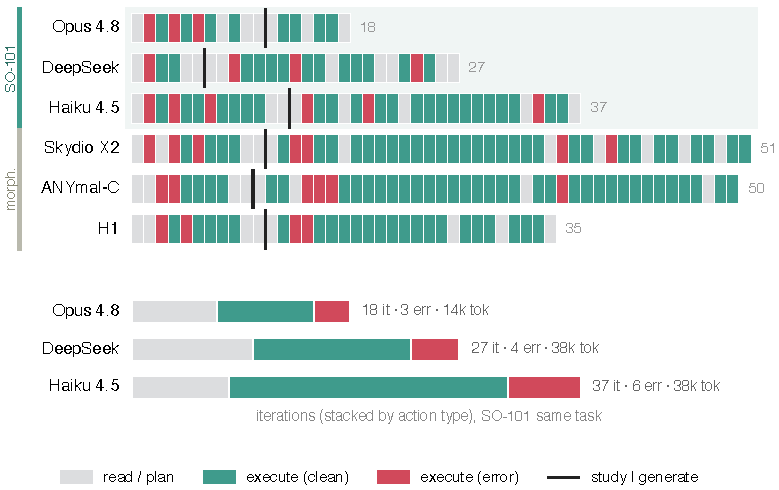
\includegraphics[width=\columnwidth]{figures/synth_trajectory.pdf}
\caption{Synthesis is a run-and-check debugging loop.
\textbf{Top:} each cell is one Generate iteration; all 24 runs needed
$\geq$1 error recovery and 73\% of iterations executed code, never
one-shot. \textbf{Bottom:} effort grows as model capability falls.
Failed-synthesis models (\S\ref{sec:cap-portability}) leave no trace.}
\label{fig:synth-traj}
\end{figure}

\subsection{Two delivery modes}
\label{sec:modes}

Generate supports two output modes. In \emph{spec mode}, the
agent writes a JSON spec (joint indices, EE link, gripper IDs) and
the runtime constructs a \texttt{Robot} from a 600-line
template for serial-arm DLS control or quadruped trot control. In
\emph{self-contained mode}, the agent writes the entire driver as
one file. Both share the same prompts, validator framework, and Demo
surface, differing only in how much code the agent authors. Spec mode is used where RL baselines must read the same
low-level joint interface (\S\ref{sec:cap-cross});
self-contained mode everywhere else. Table~\ref{tab:provenance}
(Appendix~\ref{app:onboarding}) maps every result to its mode.

\subsection{Anti-hard-coding lint}

A typical hand-built robot driver embeds structural constants in
code: joint counts, limb labels (\texttt{FL}/\texttt{FR}/
\texttt{RL}/\texttt{RR}), degree-of-freedom integers.
Auto-Adapter forces structural information to flow only from the
MJCF: Validate flags and rejects any agent-written driver that
contains hard-coded joint counts or limb labels in code paths
that index actuators. The constraint binds: first passes occasionally
contain such constants, prompting a retry. The same agent prompt
and skeleton produce driver code for a 5-joint SO-101 arm and a
12-joint ANYmal-C quadruped without modification.

\begin{algorithm}[t]
\caption{Generate phase (per-robot inner loop). Returns a
candidate driver that has passed the inner smoke check; the
outer Validate phase (\S\ref{sec:pipeline}) re-checks
independently.}
\label{alg:generate}
\begin{algorithmic}[1]
\State $\mathit{draft} \gets \textsc{LLM.WriteDriver}(\text{MJCF}, \text{study})$
\For{$\mathit{iter} = 1 \dots \texttt{max\_inner}$}
  \State Load fresh \texttt{mujoco} sim; load \texttt{draft} as Python module
  \State $(\mathit{phys}, \mathit{err}) \gets \textsc{RunSmoke}(\mathit{draft})$
  \If{$\mathit{err}$ raised}
    \State $\mathit{fb} \gets \textsc{FormatException}(\mathit{err})$
  \ElsIf{$\textsc{AllSmokeOK}(\mathit{phys})$}
    \State \Return $\mathit{draft}$
  \Else
    \State $\mathit{fb} \gets \textsc{FormatPhysDiff}(\mathit{phys}, \text{study})$
  \EndIf
  \State $\mathit{draft} \gets \textsc{LLM.Revise}(\mathit{draft}, \mathit{fb})$
\EndFor
\State \Return last $\mathit{draft}$
\end{algorithmic}
\end{algorithm}
